\documentclass{article}

\usepackage{graphicx}
\usepackage{float}

\usepackage[
	backend=bibtex
]{biblatex}
\addbibresource{refs.bib}

\title{
	Canning for Amorphous Blob Computing\\
	\small TER report
}

\author{
    Auteur :\\
    Lucas Labouret\\
    M1 QDCS, Université Paris-Saclay\\
    \small lucas.labouret@universite-paris-saclay.fr
    \and
    Encadrant :\\
    Frédéric Gruau\\
    LISN\\
    \small frederic.gruau@universite-paris-saclay.fr
}

\date{}

\begin{document}
 
\maketitle

\begin{figure}[H]
	\centering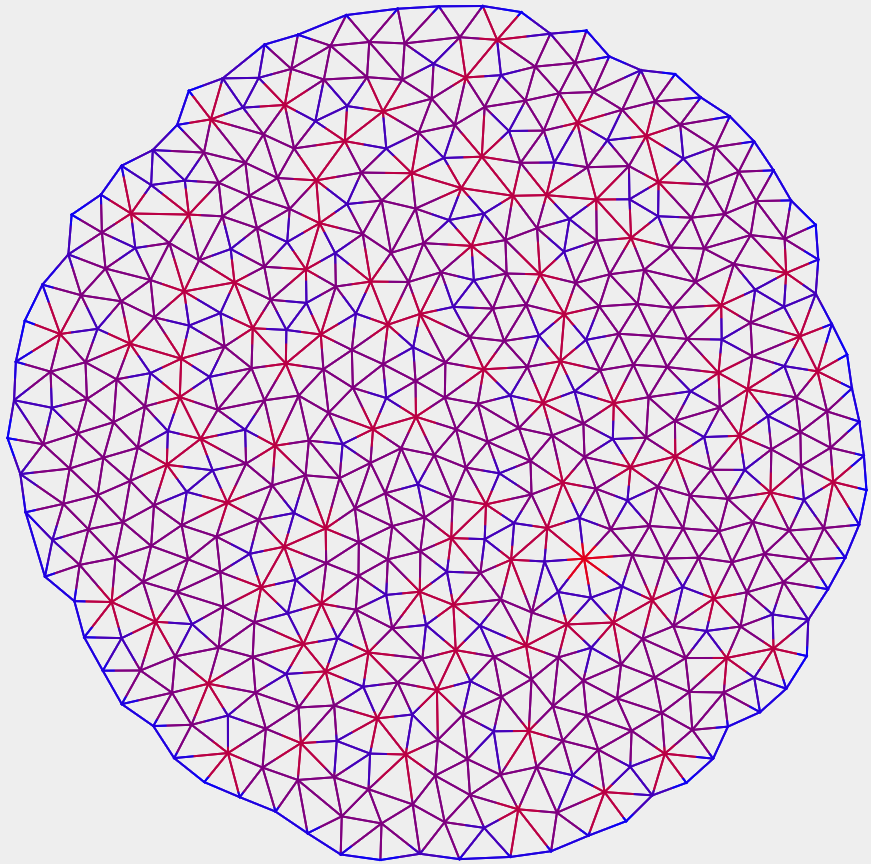
\includegraphics[width=0.9\linewidth]{assets/Circle500.png}
\end{figure}

\newpage
\tableofcontents
\newpage

\renewcommand{\thesection}{\Alph{section}}

\section{What is blob computing ?}

\subsection{Computing media}

A computing medium is a delaunay-triangulated set of points where each triangle, edge, and point is associated with a "processing element" capable of minimal computation, storing information, and communicating with its neighbors.

Computing media are the  

\subsection{An example of computation : the Voronoï diagram}

\subsection{Objective : Cannings}

\section{Preliminary work}

In this section, I detail some work I did last year during another internship with Mr Gruau to generate media with good properties. While it isn't the main focus of this year's interniship, it is what made it possible in its current form.

\subsection{Delaunay Triangulation}

\subsection{Farthest Point Optimization}

The Farthest Point Optimization algorithm \supercite{FPO} allows for the construction of the irregular yet homogeneous sets of points that we need for blob computing.

One key difference between the original article and my computing that made the implementation of FPO not-so-straightforward is the fact that the article applied the algorithm to sets of points in the unit torus, while the media use bounded subsets of the euclidean plane instead. In particular, I had to adapt the algorithm to work around the existence of a border that is not necessarily regular or convex, and that can contain fixed points that shouldn't be moved even though they can still influence the placement of other points.


\renewcommand{\thesection}{\arabic{section}}
\setcounter{section}{0}

\section{GUI}

\section{Borders and media}

\subsection{Choice of border}

\subsection{Different types of medium}

\section{Canning and evaluation}

\subsection{Partial and total cannings}

\subsection{Evaluation}

\printbibliography[heading=bibintoc]

\end{document}
